\documentclass[11pt]{article}
\usepackage[paper=letterpaper,margin=2cm]{geometry}
\usepackage{graphicx}
\usepackage[export]{adjustbox}
\usepackage{hyperref}
\usepackage{bookmark}
\usepackage{listings}
\usepackage{enumitem}
\usepackage{titlesec}
\usepackage{amsmath,amsfonts,amssymb}
\usepackage{tabularray}

\graphicspath{ {./images/} }

\hypersetup{
    colorlinks,
    citecolor=black,
    filecolor=black,
    linkcolor=black,
    urlcolor=blue
}

\lstset{
    language=C,
    basicstyle=\small\ttfamily,
    %numbers=left,
    %numberstyle=\footnotesize,
    frame=single,
    tabsize=2,
    breaklines=true,
    xleftmargin=.35em,
    xrightmargin=.35em,
    %framexleftmargin=1.6em,
    extendedchars=true,
    literate={à}{{\`a}}1 {á}{{\'a}}1 {ã}{{\~a}}1 {ç}{{\c{c}}}1 {é}{{\'e}}1 {“}{{\“}}1 {”}{{\”}}1 {ê}{{\^e}}1 {õ}{{\~o}}1 {í}{{\'i}}1 {ú}{{\'u}}1 {é }{{\'e }}2
}

\setitemize{topsep=-4pt,itemsep=0pt}
\SetTblrInner{rowsep=2pt}

\setcounter{tocdepth}{4}
\setcounter{secnumdepth}{4}

\titleformat{\paragraph}
{\normalfont\normalsize\bfseries}{\theparagraph}{1em}{}
\titlespacing*{\paragraph}
{0pt}{3.25ex plus 1ex minus .2ex}{1.5ex plus .2ex}

\begin{document}

\begin{titlepage}
    \centering
    \vspace*{4cm}
    \textbf{\LARGE Sistemas Operativos} \\[0.5cm]
    \Large Resumo \\[2cm]
    \textbf{Rafael Rodrigues} \vfill
    LEIC \\ Instituto Superior Técnico \\ 2023/2024
\end{titlepage}

\pdfbookmark[section]{\contentsname}{toc}
\tableofcontents

\setlength\parskip{1em plus 0.1em minus 0.2em}
\setlength{\parindent}{0pt}

\newpage

\section{Organização dos Sistema Operativos}

\subsection{Conceitos}

TODO

\subsection{System Calls}

TODO

\subsection{Estruturas do Sistema Operativo}

TODO

\begin{itemize}
    \item Sistemas Monolíticos
    \item Sistemas em Camadas
    \item Micro-Núcleos
\end{itemize}

\subsection{Boot}

Sequência de inicialização de um computador:
\begin{enumerate}[topsep=0pt,itemsep=0pt]
    \item A máquina recebe energia, o PC (Program Counter) aponta para um programa (firmware) na Boot ROM, normalmente uma BIOS ou UEFI.
    \item  Este programa faz algumas verificações sobre o computador (se está em condições de ser iniciado) e, de seguida, determina a localização do bootloader.
    \item  Copia o bootloader para RAM, e passa-lhe o controlo (salta).
    \item O bootloader, por sua vez, carrega o programa do núcleo em RAM e salta para a rotina de inicialização do núcleo:
          \begin{itemize}[topsep=0pt]
              \item inicializar as suas estruturas de dados
              \item copiar rotinas de tratamento de cada interrupção para RAM
              \item preencher a tabela de interrupções em RAM
              \item lançar os processos inicias do sistema, incluindo o processo de login
          \end{itemize}
\end{enumerate}

\subsection{Gestor de Processos}

TODO

\subsection{Despacho}

TODO

\begin{itemize}
    \item Se o núcleo não utilizasse uma pilha (stack) diferente da usada pelas aplicações, aplicações maliciosas poderiam manipular o estado interno do kernel.
    \item A última instrução executada pelo despacho é Return from Interrupt (RTI).
    \item A comutação entre processos implica custos maiores do que a comutação entre tarefas do mesmo processo.
    \item Um processo no estado executável executa sempre em modo núcleo antes de executar em modo utilizador.
    \item Durante a execução da chamada de sistema execl o núcleo copia os argumentos de input da execl da pilha utilizador para a pilha núcleo
    \item A escolha da min\_granularity pode afetar a latência de comutação.
    \item O processo quando é acordado por um evento necessita de verificar se a condição que levou a acordar ainda é válida senão tem de bloquear-se. Se se bloqueou com \lstinline|wait_interruptible| os \lstinline|signals| desbloqueiam o processo e não verifica se a condição de bloqueio se tornou válida
\end{itemize}

\subsection{Escalonamento (Scheduling)}

\textbf{Scheduler} - escolhe porque ordem devem correr os processos executáveis, e por quanto tempo.

\subsubsection*{Métricas}

Para o nosso escalonamento ser o melhor possível, é necessário definir métricas:
\begin{itemize}
    \item \textbf{Throughput}: número de trabalhos por hora
    \item \textbf{Turn around time}: tempo entre a submissão do trabalho e a obtenção do resultado
    \item \textbf{Utilização de CPU}: percentagem de tempo de uso do processador
    \item \textbf{Responsividade}: responder o mais rapidamente possível aos eventos desencadeados por utilizadores
    \item \textbf{Previsibilidade}: garantir que os conteúdos são carregados pelo menos a uma dada velocidade. Importante, por exemplo, para conteúdos de multimédia.
\end{itemize}

Um conceito também importante é o da prioridade de um processo, que dita a sua importância. Um processo prioritário corre com maior probabilidade que um outro. A prioridade pode ser fixa ou dinâmica.

Podemos ainda categorizar os processos em duas classes, do ponto de vista do scheduler:
\begin{itemize}
    \item \textbf{I/O bound}: fazem uso intensivo de dispositivos de entrada e saída - são interativos. \\[4pt]
          Não costumam utilizar todo o quantum que lhes é disponibilizado.
    \item \textbf{CPU bound}: fazem uso intensivo do processador. \\[4pt]
          São normalmente penalizados pelos algoritmos de escalonamento que utilizam prioridades dinâmicas
\end{itemize}

\subsubsection*{Políticas}

\begin{itemize}
    \item \textbf{Round-Robin} \\[4pt]
          Nesta política, define-se um quantum (ou time-slice) - um intervalo de tempo onde um processo está em execução. Ao fim de um quantum, chama-se o dispatcher. A implementação é trivial: uma FIFO de processos, o dispatcher faz push do processo que saiu de execução (ou de um novo que chegou) e pop daquele que vai colocar em execução. A grande desvantagem é que pode levar a tempos de resposta elevados em situações de muita carga.
    \item \textbf{Multi-lista} \\[4pt]
          Uma forma de contornar a falha do round-robin é gerir os processos em várias FIFOs - cada uma correspondente a um nível de prioridade. Faz-se pop da lista com maior prioridade primeiro, permitindo, por exemplo, que processos intensivos em IO sejam mais responsivos. Uma adição importante a este sistema é ter um quantum variável para cada lista, permitindo assim que os com maior prioridade sejam mais responsivos.
    \item \textbf{Preempção} \\[4pt]
          Retirar o CPU ao processo em execução logo que haja um mais prioritário, permitindo que os processos prioritários sejam mais responsivos. Isto é difícil de implementar, por isso, relaxa-se a definição. É então aplicada pseudo-preempção: o processo perde o CPU ao fim de um tempo
          mínimo.
\end{itemize}

\subsubsection{Gestor de Processos no Unix}

O Unix suporta dois tipos de prioridade:
\begin{itemize}
    \item Prioridades para processos em modo núcleo:
          \begin{itemize}
              \item vão de 0 a N (quanto mais pequeno, mais prioritário)
              \item são calculadas dinamicamente em função do tempo de processador utilizado
              \item escalonamento (quase) preemptivo
          \end{itemize}
    \item Prioridades para processos em modo utilizador:
          \begin{itemize}
              \item têm valores negativos (quanto mais negativo, mais prioritário)
              \item são fixas, consoante o acontecimento que o processo está a tratar;
              \item são sempre mais prioritárias que os processos em modo utilizador.
          \end{itemize}
\end{itemize}

As prioridades do utilizador seguem o seguinte algoritmo:
\begin{itemize}
    \item O CPU é sempre atribuído ao processo mais prioritário durante um quantum de 100ms (5 ticks)
    \item Round-Robin entre os processos mais prioritários
    \item A cada segundo (50 ticks) as prioridades são recalculadas de acordo com a seguinte fórmula:
\end{itemize}
\begin{equation*}
    prioridade = prioridade_{base} + \frac{CPUtime}{2}
\end{equation*}
\begin{equation*}
    CPUtime = \frac{CPUtime}{2}
\end{equation*}

Chamadas de sistema importantes relacionadas com o scheduling:
\begin{itemize}
    \item \lstinline|nice(int val)| : Muda o valor \lstinline|nice| de um processo
          \begin{itemize}[topsep=-2pt]
              \item Adiciona o valor \lstinline|val| ao \lstinline|nice| atual do processo, tornando-o menos prioritário se \lstinline|val| for positivo.
              \item Apenas superuser pode invocar com \lstinline|val| negativo, tornando o processo mais prioritário
          \end{itemize}
    \item \lstinline|getpriority(int which, int id)|: retorna prioridade de um processo ou grupo de processos
    \item \lstinline|setpriority(int which, int id, int prio)|: altera prioridade do processo ou grupo de processos
\end{itemize}

O Gestor de Processos no Unix recalcula a prioridade de todos os processos a cada segundo, ou seja, ao aumentar do número de processos o algoritmo de escalonamento Unix torna-se pouco eficiente.

\subsubsection{Gestor de Processos no Linux}

No Linux, o tempo é dividido em épocas. Uma época acaba quando todos os processos usaram o seu quantum disponível ou estão bloqueados.

O quantum e prioridade são atribuídos no início de cada época por:
\begin{equation*}
    quantum = quantum_{base} +
    \frac{quantum_{por\ usar\ epoca\ anterior}}{2}
\end{equation*}
\begin{equation*}
    prioridade = prioridade_{base} + quantum_{por\ usar\ epoca\ anterior} - nice
\end{equation*}

O valor do quantum pode ser mudado com chamadas de sistema.

As prioridades mais importantes são as com valor mais elevado.

\subsubsection{Completely Fair Scheduler (CFS)}

O CFS é o scheduler atualmente utilizado pelo Linux. Adiciona a cada processo um novo atributo \lstinline|vruntime| que representa o seu tempo acumulado de execução em modo utilizador.

Um novo processo inicia com \lstinline|vruntime| igual ao mínimo entre o \lstinline|vruntime| dos processos ativos. Quando o processo perde CPU, o seu \lstinline|vruntime| é incrementado com o tempo executado nesse quantum.

Os processos executáveis são guardados numa red-black tree ordenada por \lstinline|vruntime|, que permite encontrar o processo mais prioritário em O(log n). O processo mais prioritário é o com menor \lstinline|vruntime|.

\newpage

\section{Sistemas de Ficheiros}

\subsection{Ficheiros}

Definimos um ficheiro como uma coleção de dados persistentes, geralmente relacionados, identificados por um nome.

Os vários ficheiros de um certo sistema estão normalmente organizados num sistema de ficheiros.

\subsubsection{Nomes}

Para aceder a um ficheiro temos de saber como referir ao SO a qual ficheiro estamos a querer aceder.

\begin{itemize}
    \item Nomes Absolutos
          \begin{itemize}
              \item Caminho de acesso desde a raiz (root, normalmente denominado /)
          \end{itemize}
    \item Nomes Relativos
          \begin{itemize}
              \item Caminho de acesso a partir do diretório corrente
              \item O diretório corrente é mantido para cada processo como parte do seu contexto
          \end{itemize}
\end{itemize}

\subsection{Links}

Um ficheiro pode ser conhecido por vários nomes, ou seja, é possível querermos associar um dado conjunto de dados a mais que um nome (eventualmente em diretorias diferentes).

\begin{itemize}
    \item Hard link
          \begin{itemize}
              \item Corresponde ao conceito de cópia de um ficheiro (sem cópia real dos dados).
              \item Se apagarmos um ficheiro com vários hard links, o ficheiro continua a existir. Só será removido quando o ultimo hard link for apagado.
          \end{itemize}
    \item Symbolic link
          \begin{itemize}
              \item É um ficheiro (de tipo diferente) que contem o caminho de acesso para o ficheiro original.
              \item Quando se apaga um symbolic link para um ficheiro, o ficheiro nunca é apagado.
              \item Se o ficheiro original for apagado o link fica quebrado.
          \end{itemize}
\end{itemize}

\subsubsection{Programar com Ficheiros}

TODO

\subsection{Organização do Disco}

Um disco está dividido em partições (e um sector de 512B, o MBR). Para qualquer partição do disco, existe sempre um \lstinline|boot block|, que contém código (instruções) que vai ser carregado para RAM.

O grande desafio do sistema de ficheiros é conseguir organizar o volume para (de uma forma eficiente) armazenar os dados.

\subsubsection{Organização em Lista e Diretório}

\begin{itemize}
    \item \textbf{Organização em Lista} \\[4pt]
          Neste modelo cada ficheiro é um nó numa lista ligada (os campos sendo o nome, o tamanho, o ficheiro seguinte e os dados)
          \begin{itemize}
              \item \textbf{Vantagens}: forma simples e compacta de organizar um sistema de ficheiros
              \item \textbf{Desvantagens}: tempo necessário para localizar um ficheiro, fragmentação de memória
          \end{itemize}
    \item \textbf{Organização em Diretório} \\[4pt]
          Neste modelo os metadados (nome e dimensão) são compactados numa diretoria, mantendo referências para a localização dos dados.
          \begin{itemize}
              \item \textbf{Vantagens}: aumenta a eficiência da procura de um ficheiro pelo seu nome
              \item \textbf{Desvantagens}: perda de funcionalidade para diminuir a fragmentação externa usando blocos
          \end{itemize}
\end{itemize}

\subsubsection{Sistema de Ficheiros do CP/M e MS-DOS}

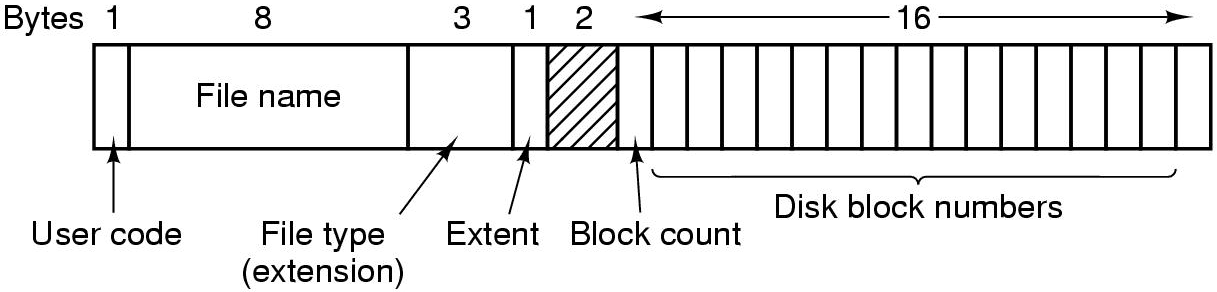
\includegraphics[scale=0.35,center]{cpm.png}

O CP/M é baseado na organização em diretório, cada entrada do diretório do sistema de ficheiros tinha 32B. Como cada bloco tinha 1 KB, os ficheiros tinham, no máximo, 16 KB.

Para aumentar a dimensão máxima do ficheiro podemos:
\begin{itemize}
    \item aumentar o mapa de blocos, ou seja, tamanho das entradas (ineficiente para ficheiros pequenos)
    \item aumentar o tamanho dos blocos (maior fragmentação interna)
\end{itemize}

O MS-DOS possui uma estrutura de sistema de ficheiros semelhante ao CP/M, mas em vez de um mapa de blocos por ficheiro, no MS-DOS existe uma tabela de blocos global partilhada por todos os ficheiros.

\subsubsection{Sistema de File Allocation Table}

Num sistema de ficheiros FAT (designado FAT-Y, para $n$=Y), a partição contém três secções distintas:
\begin{itemize}
    \item A tabela de alocação: um vetor com, no máximo, $2^n$ inteiros de $n$ bits. Cada entrada contém:
          \begin{itemize}[topsep=-2pt]
              \item \lstinline|0| se o bloco com o esse índice está livre
              \item \lstinline|max| se esse é o último bloco de um cadeia de blocos de um ficheiro
              \item \lstinline|x| indica qual é o índice do próximo bloco com dados relativos um ficheiro
          \end{itemize}
    \item Um diretório com os nome do ficheiro e um inteiro correspondente a um índice da FAT, para cada ficheiro presente no sistema.
    \item uma secção com o espaço restante dividido em blocos, de igual dimensão, para conter os dados dos ficheiros.
\end{itemize}

O tamanho máximo de um ficheiro em FAT-Y é de $2^{Y-1}$ blocos.

\textbf{Desvantagens}:
\begin{itemize}
    \item Elevada dimensão da FAT quando os discos têm dimensões muito grandes.
    \item Não é possível manter tabelas desta dimensão em RAM, sendo preciso ler a FAT do disco, o que prejudica muito o acesso à cadeia de blocos de um ficheiro.
\end{itemize}

\subsubsection{Organização com i-nodes}

Este sistema cria uma estrutura de dados, um i-node, com informação relevante sobre o ficheiro (tipo de ficheiro, dono, datas de últimos acessos, permissões, dimensão, localizações dos blocos de dados).

Isto permite organizar o sistema de ficheiros como uma árvore ou hash table de i-nodes, e que várias entradas numa diretoria apontem para o mesmo ficheiro (referenciam o mesmo i-node).

Em cada partição, cada ficheiro é identificado univocamente pelo i-number (número do inode). Assim, as diretorias têm que ser apenas um mapeamento entre nomes e i-numbers.

Num descritor do volume, podemos encontrar a localização de tabela de i-nodes e a tabela de alocação. Dada a importância do descritor de volume (ou super-bloco), este tipicamente está replicado.

A tabela de alocação é um bitmap que indica se um bloco está livre ou não.

\subsubsection{Sistema de Ficheiros EXT}

TODO

\begin{itemize}
    \item No Ext3 quer os ficheiros quer os diretórios têm um i-node associado que descreve os respetivos metadados.
    \item No Ext3 os diretórios guardam a associação entre os nomes dos ficheiros e os respetivos i-nodes (i-number)
    \item O número de ficheiros guardados num sistema de ficheiros Ext3 não pode ultrapassar o número de entradas na tabela de i-nodes
\end{itemize}

A dimensão máxima de um ficheiro é dado por: \\[8pt]
\begin{minipage}{0.5\textwidth}
    \begin{equation*}
        t_{max} = B \times \left[12 + \frac{B}{R} + \left(\frac{B}{R}\right)^2
            + \left(\frac{B}{R}\right)^3 \right]\
    \end{equation*}
\end{minipage}
\begin{minipage}{0.495\textwidth}
    $B$ - tamanho do bloco em bytes \\
    $R$ - tamanho da referência para um bloco em bytes
\end{minipage}

\subsubsection{Estruturas de Suporte}

TODO

\newpage

\section{Processos e Tarefas}

\subsection{Processos}

Um processo é uma entidade ativa controlada por um programa e que necessita de um processador para poder executar-se. Cada processo tem:
\begin{itemize}
    \item Espaço de Endereçamento
          \begin{itemize}
              \item Código do programa
              \item Heap - Zona para os dados, variáveis globais e alocação
                    dinâmica de estruturas de dados
              \item Stack
          \end{itemize}
    \item Reportório de Instruções
          \begin{itemize}
              \item Instruction set da máquina do processador
              \item Instruções do sistema operativo
          \end{itemize}
    \item Estado interno
          \begin{itemize}
              \item Guardam components como program counter, stack pointer, status register, ...
          \end{itemize}
\end{itemize}

Os processos relacionam-se de forma hierárquica, um novo processo herda grande parte do contexto do processo pai.

Se um processo pai termina, os seus sub-processos continuam a executar-se e são adotados pelo processo de inicialização (\lstinline|pid = 1|).

\subsubsection{Criação do Processo}

\begin{enumerate}[topsep=0pt,itemsep=0pt]
    \item Reserva-se uma entrada na tabela \lstinline|proc| (verificando se o utilizador não excedeu o número máximo de processos).
    \item Atribui-se um \lstinline|pid|.
    \item Copia-se a imagem do processo pai (com copy-on-write, para aumentar a performance).
\end{enumerate}

\begin{tblr}{width=\linewidth,colspec={ | X[l,m] | }}
    \hline
    \lstinline|pid_t fork()|                                  \\\hline
    \lstinline|Retorna 0 ao processo filho|                   \\
    \lstinline|Retorna pid do processo filho ao processo pai| \\
    \lstinline|Retorna -1 em caso de erro|                    \\\hline
\end{tblr}

\subsubsection{Terminação do Processo}

\begin{enumerate}[topsep=0pt,itemsep=0pt]
    \item Executar funções registadas pelo \lstinline|atexit|.
    \item Libertar recursos (ficheiros, diretoria, memória). \textbf{Não} elimina a \lstinline|task_struct|.
    \item Atualizar o ficheiro que regista a utilização do processador, memória e IO.
    \item Enviar o sinal \lstinline|SIGCHLD| ao pai.
\end{enumerate}

\begin{tblr}{width=\linewidth,colspec={ | X[l,m] | }}
    \hline
    \lstinline|void exit(int status)|                         \\\hline
    \lstinline|status: valor que é retornado ao processo pai| \\\hline
\end{tblr}

Entre \lstinline|exit| e \lstinline|wait|, processo filho diz-se zombie, só depois de \lstinline|wait| o processo é totalmente esquecido. \\
Enquanto procura filhos zombies o processo pai bloqueia.

\begin{tblr}{width=\linewidth,colspec={ | X[l,m] | }}
    \hline
    \lstinline|int wait(int *status)|                                             \\\hline
    \lstinline|status: estado que é retornado ao processo pai pelo filho no exit| \\\hline
    \lstinline|Retorna o pid do processo terminado|                               \\\hline
\end{tblr}

\subsubsection{Substituição do Processo}

O \lstinline|exec()| carrega um novo programa num processo já existente, em que:
\begin{enumerate}[topsep=0pt]
    \item Verifica que o processo existe e é executável
    \item Copia os argumentos do exec para a pilha do núcleo (a pilha do utilizador vai ser destruída)
    \item Liberta os dados referentes ao programa antigo
    \item Reserva dados para o novo programa
    \item Carrega o executável.
    \item Copia os argumentos para a pilha do utilizador
\end{enumerate}

O código a seguir a chamada à \lstinline|exec()| só é executado caso a chamada sistema falhar. A área de dados e a pilha do programa atual são libertados caso a \lstinline|exec()| tenha sucesso.

\subsubsection{Exemplo}

\begin{lstlisting}
main () {
    int pid, status;
    pid = fork();
    if(pid == 0) {
        /* algoritmo do processo filho */
        exit(0);
    } else {
        /* o processo pai bloqueia à espera da terminação do processo filho */
        pid = wait(&status);
    }
}
\end{lstlisting}

\newpage

\subsection{Tarefas}

Mecanismo simples para criar fluxos de execução independentes, partilhando um contexto comum.

Tarefas do mesmo processo partilham o código, o heap (variáveis globais e variáveis dinamicamente alocadas) e atributos do processo. \textbf{Não partilham} a stack, o estado dos registos do processador e os seus atributos específicos.

Vantagens:
\begin{itemize}
    \item Criação e comutação entre tarefas do mesmo processo é mais leve.
    \item Tarefas podem comunicar através de memória partilhada.
\end{itemize}

Desvantagens:
\begin{itemize}
    \item Não podem executar diferentes binários em paralelo.
    \item Não permitem o isolamento de bugs.
\end{itemize}

\subsubsection{Interface POSIX}

\begin{tblr}{width=\linewidth,colspec={ | X[l,m] | }}
    \hline
    \centering Criar uma tarefa                                                                                    \\\hline
    \lstinline|int pthread_create(pthread_t *tid, const pthread_attr_t *attr, void *(*routine)(void*), void *arg)| \\\hline
    \lstinline|pid: apontador para o identificador da tarefa|                                                      \\
    \lstinline|attr: atributos da tarefa|                                                                          \\
    \lstinline|routine: função a executar|                                                                         \\
    \lstinline|arg: ponteiro para argumentos da função|                                                            \\\hline
    \lstinline|Retorna 0 em caso de sucesso|                                                                       \\
    \lstinline|Retorna -1 em caso de erro|                                                                         \\\hline
\end{tblr}

\begin{tblr}{width=\linewidth,colspec={ | X[l,m] | }}
    \hline
    \centering Termina a tarefa chamadora                   \\\hline
    \lstinline|void pthread_exit(void *retval)|             \\\hline
    \lstinline|retval: ponteiro para valor a ser retornado| \\\hline
\end{tblr}

\begin{tblr}{width=\linewidth,colspec={ | X[l,m] | }}
    \hline
    \centering Tarefa chamadora espera até a tarefa indicada ter terminado \\\hline
    \lstinline|int pthread_join(pthread_t thread, void **retval)|          \\\hline
    \lstinline|thread: tarefa pela qual tarefa chamadora espera|           \\
    \lstinline|retval: ponteiro retornado pela tarefa terminada|           \\\hline
\end{tblr}

\newpage

\subsection{Memória Partilhada}

\subsubsection{Secção Crítica}

Uma \textbf{secção crítica} é um bloco que deve ser executado de forma \textbf{indivisível} ou \textbf{atómica}.

Em programação concorrente, sempre que atividades concorrentes acedem a recursos
partilhados, \textbf{é necessário efetuá-lo dentro de uma secção crítica}.

As secções críticas são delimitadas por um fecho e uma correspondente libertação para outras tarefas. Dizemos, para estas ações, que são o \textbf{lock} e \textbf{unlock} da secção crítica. Para este fim, utilizamos os \textbf{trincos lógicos}.

\subsubsection{Mutex}

Uma secção crítica fechada por um mutex só pode acedida quando este for aberto.

O uso de trincos diferentes para secções críticas independentes maximiza o paralelismo do programa.

\begin{tblr}{width=\linewidth,colspec={ | X[l,m] | }}
    \hline
    \centering Inicializar um trinco             \\\hline
    \lstinline|int pthread_mutex_init(pthread_mutex_t *mutex, pthread_mutexattr_t
    *attr)|                                      \\\hline
    \lstinline|mutex: trinco a ser inicializado| \\
    \lstinline|attr: atributos do trinco|        \\\hline
    \lstinline|Retorna 0 em caso de sucesso|     \\
    \lstinline|Retorna -1 em caso de erro|       \\\hline
\end{tblr}

\begin{tblr}{width=\linewidth,colspec={ | X[l,m] | }}
    \hline
    \centering Fechar ou abrir um trinco                           \\\hline
    \lstinline|int pthread_mutex_[un]lock(pthread_mutex_t *mutex)| \\\hline
    \lstinline|mutex: trinco que será locked ou unlocked|          \\\hline
    \lstinline|Retorna 0 em caso de sucesso|                       \\
    \lstinline|Retorna -1 em caso de erro|                         \\\hline
\end{tblr}

\begin{tblr}{width=\linewidth,colspec={ | X[l,m] | }}
    \hline
    \centering Tentar bloquear um trinco                          \\\hline
    \lstinline|int pthread_mutex_trylock(pthread_mutex_t *mutex)| \\\hline
    \lstinline|mutex: trinco que se tentará bloquear|             \\\hline
    \lstinline|Retorna 0 em caso de sucesso|                      \\
    \lstinline|Retorna -1 em caso de erro|                        \\\hline
\end{tblr}

\begin{tblr}{width=\linewidth,colspec={ | X[l,m] | }}
    \hline
    \centering Bloquear uma trinco por um dado tempo               \\\hline
    \lstinline|int pthread_mutex_timedlock(pthread_mutex_t *mutex, const struct
    timespec *timeout)|                                            \\\hline
    \lstinline|mutex: trinco a ser inicializado|                   \\
    \lstinline|timeout: estrutura que indica o tempo a fazer lock| \\\hline
    \lstinline|Retorna 0 em caso de sucesso|                       \\
    \lstinline|Retorna -1 em caso de erro|                         \\\hline
\end{tblr}

\begin{tblr}{width=\linewidth,colspec={ | X[l,m] | }}
    \hline
    \centering Destruir um trinco                                 \\\hline
    \lstinline|int pthread_mutex_destroy(pthread_mutex_t *mutex)| \\\hline
    \lstinline|mutex: trinco a ser destruído|                     \\\hline
    \lstinline|Retorna 0 em caso de sucesso|                      \\
    \lstinline|Retorna -1 em caso de erro|                        \\\hline
\end{tblr}

\subsubsection{Trinco de Leitura-Escrita}

Permitem fechar a secção crítica para ler ou para escrever.
\begin{itemize}
    \item Os escritores só podem aceder em exclusão mútua.
    \item Os leitores podem aceder simultaneamente com outros leitores, mas em exclusão mútua com os escritores.
\end{itemize}

Vantajoso quando acessos de leitura às secções críticas são dominantes.

\begin{tblr}{width=\linewidth,colspec={ | X[l,m] | }}
    \hline
    \centering Fechar um trinco para leitura                      \\\hline
    \lstinline|int pthread_rwlock_rdlock(pthread_rwlock_t *lock)| \\\hline
    \lstinline|lock: trinco que será fechado|                     \\\hline
    \lstinline|Retorna 0 em caso de sucesso|                      \\
    \lstinline|Retorna -1 em caso de erro|                        \\\hline
\end{tblr}

\begin{tblr}{width=\linewidth,colspec={ | X[l,m] | }}
    \hline
    \centering Fechar um trinco para escrita                      \\\hline
    \lstinline|int pthread_rwlock_wrlock(pthread_rwlock_t *lock)| \\\hline
    \lstinline|lock: trinco que será fechado|                     \\\hline
    \lstinline|Retorna 0 em caso de sucesso|                      \\
    \lstinline|Retorna -1 em caso de erro|                        \\\hline
\end{tblr}

\begin{tblr}{width=\linewidth,colspec={ | X[l,m] | }}
    \hline
    \centering Abrir um trinco                                    \\\hline
    \lstinline|int pthread_rwlock_unlock(pthread_rwlock_t *lock)| \\\hline
    \lstinline|lock: trinco que será aberto|                      \\\hline
    \lstinline|Retorna 0 em caso de sucesso|                      \\
    \lstinline|Retorna -1 em caso de erro|                        \\\hline
\end{tblr}

As funções de inicialização (\lstinline|pthread_rwlock_init|) e de destruição (\lstinline|pthread_rwlock_destroy|) são semelhantes às dos mutexes.

\subsubsection{Semáforos}

Um semáforo é uma primitiva de sincronização mais genérica, que pode ser visto como um contador atómico. É inicializado com o número de threads que podem entrar numa secção crítica (ao entrarem fazem \lstinline|sem_wait| e decrementam o contador) e ao sair fazem \lstinline|sem_post| (incrementando o contador).

\begin{itemize}
    \item Para bloquear uma tarefa T1 até o acontecimento de um evento detetado pela tarefa T2, pode-se usar um semáforo inicializado com 0, onde T1 espera e T2 assinala.
\end{itemize}

TODO

\subsubsection{Variáveis de Condição}

TODO

\newpage

\subsection{Troca de Mensagem}

\subsubsection{Pipes}

Um pipe é um canal byte stream, unidirecional, que liga dois processos. Os descritores de um pipe são semelhantes aos de um ficheiro, mas são internos ao processo e podem ser transmitidos aos processos filhos através do mecanismo de herança.

As duas extremidades de um pipe criado pelo pai ficam automaticamente abertas no processo filho quando se efetuar o fork.

\begin{tblr}{width=\linewidth,colspec={ | X[l,m] | }}
    \hline
    \centering Criar um Pipe                          \\\hline
    \lstinline|int pipe(int *fds)|                    \\\hline
    \lstinline|fds[0]: descritor aberto para leitura| \\
    \lstinline|fds[1]: descritor aberto para escrita| \\\hline
    \lstinline|Retorna 0 em caso de sucesso|          \\
    \lstinline|Retorna -1 em caso de erro|            \\\hline
\end{tblr}

\subsubsection{Named Pipes}
Um named pipe é, como o nome indica, um pipe identificado por um nome. Permite que dois processos que não têm qualquer relação hierárquica comuniquem. Um named pipe comporta-se externamente como um ficheiro, existindo uma entrada na diretoria correspondente, mas \textbf{não é persistente}.

Um processo que abra uma extremidade do canal \textbf{bloqueia} até que pelo menos 1 processo tenha aberto a outra extremidade.

\begin{tblr}{width=\linewidth,colspec={ | X[l,m] | }}
    \hline
    \centering Criar um Named Pipe                            \\\hline
    \lstinline|int mkfifo(const char *pathname, mode_t mode)| \\\hline
    \lstinline|pathname: caminho do pipe|                     \\
    \lstinline|mode: permissões do ficheiro|                  \\\hline
    \lstinline|Retorna 0 em caso de sucesso|                  \\
    \lstinline|Retorna -1 em caso de erro|                    \\\hline
\end{tblr}

\begin{tblr}{width=\linewidth,colspec={ | X[l,m] | }}
    \hline
    \centering Eliminar um Named Pipe            \\\hline
    \lstinline|int unlink(const char *pathname)| \\\hline
    \lstinline|pathname: caminho do pipe|        \\\hline
    \lstinline|Retorna 0 em caso de sucesso|     \\
    \lstinline|Retorna -1 em caso de erro|       \\\hline
\end{tblr}

\subsubsection*{Exemplo}

\begin{minipage}[t]{0.5\textwidth}
    \begin{lstlisting}
/* Cliente */

main() {
    int fcli, fsrv;
    char buf[BUFSIZE];

    if((fsrv = open("/tmp/server", O_WRONLY)) < 0) exit(1);
    if((fcli = open("/tmp/client", O_RDONLY)) < 0) exit(1);

    /* produce message */
    write(fsrv, buf, strlen(buf));

    read(fcli, buf, BUFSIZE);
    /* process message */

    close(fsrv);
    close(fcli);
}
    \end{lstlisting}
\end{minipage}
\begin{minipage}[t]{0.5\textwidth}
    \begin{lstlisting}
/* Servidor */

main () {
    int fcli, fsrv;
    char buf[BUFSIZE];

    unlink("/tmp/servidor");
    unlink("/tmp/cliente");

    if(mkfifo("/tmp/server", 0777) < 0) exit (1);
    if(mkfifo("/tmp/client", 0777) < 0) exit (1);

    if((fsrv = open("/tmp/server", O_RDONLY)) < 0) exit(1);
    if((fcli = open("/tmp/client", O_WRONLY)) < 0) exit(1);

    for (;;) {
        if(read(fsrv, buf, BUFSIZE) <= 0) break;
        /* process message */
        
        /* produce message */
        write (fcli, buf, strlen(buf));
    }

    close(fsrv);
    close(fcli);

    unlink("/tmp/server");
    unlink("/tmp/client");
}
    \end{lstlisting}
\end{minipage}

\subsubsection{Sockets}

Um socket é uma extremidade de um canal de comunicação, um socket pode ter um nome (socket address) associado para permitir que outros processos o referenciem. Num exemplo com dois processos a comunicar, existirão (pelo menos) dois sockets.

\begin{tblr}{width=\linewidth,colspec={ | X[l,m] | }}
    \hline
    \centering Criar um socket                                       \\\hline
    \lstinline|int socket(int domain, int type, int protocol)|       \\\hline
    \lstinline|domain: domínio da comunicação (AF_UNIX, AF_INET)|    \\
    \lstinline|type: tipo de socket (SOCK_STREAM, SOCK_DGRAM)|       \\\hline
    \lstinline|Retorna o identificador do socket em caso de sucesso| \\
    \lstinline|Retorna -1 em caso de erro|                           \\\hline
\end{tblr}

\begin{tblr}{width=\linewidth,colspec={ | X[l,m] | }}
    \hline
    \centering Associar um nome (endereço de comunicação) a um socket já criado \\\hline
    \lstinline|int bind(int sockfd, struct sockaddr *addr,
    socklen_t addrlen)|                                                         \\\hline
    \lstinline|sockfd: file descriptor do socket|                               \\
    \lstinline|addr: endereço a associar ao socket|                             \\
    \lstinline|addrlen: tamanho da estrutura apontada por addr|                 \\\hline
    \lstinline|Retorna 0 em caso de sucesso|                                    \\
    \lstinline|Retorna -1 em caso de erro|                                      \\\hline
\end{tblr}

\subsubsection*{Sockets sem Ligação (datagram)}

\begin{itemize}
    \item Modelo de comunicação tipo correio.
    \item Canal sem ligação, bidirecional, não fiável, interface tipo mensagem.
\end{itemize}

\begin{tblr}{width=\linewidth,colspec={ | X[l,m] | }}
    \hline
    \centering Envia uma mensagem para o endereço especificado  \\\hline
    \lstinline|int sendto(int sockfd, char *msg, int length, int flag,
    struct sockaddr *dest, int addrlen)|                        \\\hline
    \lstinline|sockfd: file descriptor do socket|               \\
    \lstinline|msg: mensagem a enviar|                          \\
    \lstinline|length: tamanho da mensagem|                     \\
    \lstinline|dest: endereço do socket de destino|             \\
    \lstinline|addrlen: tamanho da estrutura apontada por dest| \\\hline
    \lstinline|Retorna o número de caracteres enviados|         \\
    \lstinline|Retorna -1 em caso de erro|                      \\\hline
\end{tblr}

\begin{tblr}{width=\linewidth,colspec={ | X[l,m] | }}
    \hline
    \centering Recebe uma mensagem e devolve o endereço do emissor \\\hline
    \lstinline|int recvfrom(int sockfd, char *msg, int length, int flag,
    struct sockaddr *orig, int *addrlen)|                          \\\hline
    \lstinline|sockfd: file descriptor do socket|                  \\
    \lstinline|msg: mensagem a receber|                            \\
    \lstinline|length: tamanho da mensagem|                        \\
    \lstinline|orig: endereço do socket de origem|                 \\
    \lstinline|addrlen: tamanho da estrutura apontada por orig|    \\\hline
    \lstinline|Retorna o número de caracteres recebidos|           \\
    \lstinline|Retorna -1 em caso de erro|                         \\\hline
\end{tblr}

\subsubsection*{Sockets com Ligação (stream)}

\begin{itemize}
    \item Modelo de comunicação tipo diálogo.
    \item Canal com ligação, bidirecional, fiável, interface tipo sequência de octetos.
\end{itemize}

É estabelecido um canal de comunicação entre o processo cliente e o servidor. O servidor pode gerir múltiplos clientes, mas dedica a cada um deles uma atividade independente. O servidor pode ter uma política própria para atender os clientes.

\begin{tblr}{width=\linewidth,colspec={ | X[l,m] | }}
    \hline
    \centering Indica que se vão receber ligações neste socket (Server) \\\hline
    \lstinline|int listen (int sockfd, int backlog)|                    \\\hline
    \lstinline|sockfd: file descriptor do socket|                       \\
    \lstinline|backlog: número máximo de conexões em espera|            \\\hline
    \lstinline|Retorna 0 em caso de sucesso|                            \\
    \lstinline|Retorna -1 em caso de erro|                              \\\hline
\end{tblr}

\begin{tblr}{width=\linewidth,colspec={ | X[l,m] | }}
    \hline
    \centering Estabelece uma ligação (Client)                  \\\hline
    \lstinline|int connect(int sockfd, struct sockaddr *addr,
    socklen_t addrlen)|                                         \\\hline
    \lstinline|sockfd: file descriptor do socket|               \\
    \lstinline|addr: endereço do socket a conectar|             \\
    \lstinline|addrlen: tamanho da estrutura apontada por addr| \\\hline
    \lstinline|Retorna 0 em caso de sucesso|                    \\
    \lstinline|Retorna -1 em caso de erro|                      \\\hline
\end{tblr}

\begin{tblr}{width=\linewidth,colspec={ | X[l,m] | }}
    \hline
    \centering Aceita uma ligação (Server)                                  \\\hline
    \lstinline|int accept(int sockfd, struct sockaddr *addr, int *addrlen)| \\\hline
    \lstinline|sockfd: file descriptor do socket|                           \\
    \lstinline|addr: endereço do socket que se conecta|                     \\
    \lstinline|addrlen: tamanho da estrutura apontada por addr|             \\\hline
    \lstinline|Retorna o identificador do socket aceite em caso de sucesso| \\
    \lstinline|Retorna -1 em caso de erro|                                  \\\hline
\end{tblr}

É possível um servidor fazer espera múltipla usando o \lstinline|select|. Esta função bloqueia o processo até que um descritor tenha um evento associado ou expire o alarme.

\begin{tblr}{width=\linewidth,colspec={ | X[l,m] | }}
    \hline
    \lstinline|int select(int nfds, fd_set *read, fd_set *write,
    fd_set *error, struct timeval *timeout)|                   \\\hline
    \lstinline|nfds: número de file descriptors|               \\
    \lstinline|read: conjunto de file descriptors de leitura|  \\
    \lstinline|write: conjunto de file descriptors de escrita| \\
    \lstinline|error: conjunto de file descriptors de erro|    \\
    \lstinline|timeout: intervalo de espera|                   \\\hline
    \lstinline|Retorna número de bits em caso de sucesso|      \\
    \lstinline|Retorna -1 em caso de erro|                     \\\hline
\end{tblr}

\newpage

\subsubsection*{Exemplo}

\begin{lstlisting}
int main() {
    int server_fd, client_fd;
    struct sockaddr_in addr;
    socklen_t addrlen = sizeof(addr);
    
    if ((server_fd = socket(AF_INET, SOCK_STREAM, 0)) < 0) {
        exit(0);
    }
    
    /* set socket options and address... */
    
    if (bind(server_fd, (struct sockaddr*) &addr, sizeof(addr)) < 0) {
        exit(0);
    }

    if (listen(server_fd, 3) < 0) {
        exit(0);
    }

    client_fd = accept(server_fd, (struct sockaddr*) &addr, &addrlen)
    if (client_fd < 0) {
        exit(0);
    }

    int n = read(client_fd, buffer, BUFSIZE);
    /* do something with buffer */

    /* write response to buffer*/
    write(client_fd, buffer, strlen(buffer));
    
    close(client_fd);   /* closing the connected socket */
    close(server_fd);   /* closing the listening socket */

    return 0;
}
\end{lstlisting}

\subsection{Sinais}

TODO

Diferentes semânticas dos signals:
\begin{itemize}
    \item System V
          \begin{itemize}
              \item A associação de uma rotina a um signal é apenas efetiva para uma ativação
              \item Depois de receber o signal, o tratamento passa a ser novamente o por omissão
              \item Necessário restabelecer a associação na primeira linha da rotina de tratamento \\
                    (problema se houver receção sucessiva de signals)
          \end{itemize}
    \item BSD
          \begin{itemize}
              \item Associação signal-rotina \textbf{não} é desfeita após ativação
              \item A receção de um novo signal é inibida durante a execução da rotina de tratamento
          \end{itemize}
\end{itemize}

\begin{itemize}
    \item É uma rotina normal que fica referenciada na tabela de tratamento de signals do processo. Quando o processo vai passar de modo núcleo a modo utilizador, é testado se existe um signal pendente e por manipulação dos stacks núcleo e utilizador a rotina é posta a correr em modo utilizador
    \item Um processo pode ter associado um tratamento por omissão para todos os signals
\end{itemize}

\newpage

\section{Gestão de Memória}

O objetivo da gestão de memória é gerir o espaço de endereçamento dos processos, assegurando que cada processo dispõe da memória que precisa, garantir que cada processo só acede à memória a que tem direito e otimizar desempenho dos acessos.

\subsection{Gestor de Memória}

\textbf{Espaço de Endereçamento} - Conjunto de endereços de memória disponíveis para um processo.

O processo endereça a memória física. Esta abordagem é feita tipicamente em sistemas embebidos (e em arquiteturas antigas). No entanto, coloca problemas de portabilidade e de concorrência.

\subsection{Endereçamento Virtual}

Neste modelo, o espaço de endereçamento é virtual, logo é feita uma tradução para os endereços reais.

\subsubsection{Segmentação}

A segmentação consiste na divisão dos programas em segmentos lógicos que refletem a sua estrutura funcional (rotinas, módulos, código, dados, pilha, etc).

Através da segmentação, podemos carregar segmentos mais eficientemente e proteger os segmentos. Existe uma tabela de segmentos que faz a tradução para a memória real.

Em sistemas segmentados, um endereço virtual é um par (segmento, deslocamento) em que segmento define uma entrada na tabela de segmentos. Uma entrada da tabela de segmentos é constituída por:

\begin{tblr}{colspec={ | Q[l,m] | Q[l,m] |}}
    \hline
    P      & Indica se o segmento correspondente a esta entrada está presente na memória principal \\\hline
    Prot   & Definem as proteções do segmento em causa                                             \\\hline
    Limite & Indica o número de endereços que constituem este segmento                             \\\hline
    Base   & Endereço na memória principal em que está a informação relativa ao segmento           \\\hline
\end{tblr}

\subsubsection{Páginação}

A paginação consiste em dividir a memória em blocos de tamanho fixo, chamados páginas, que são a unidade de carregamento entre a memória primária e secundária.

Em sistemas paginados, um endereço virtual será então um par (página, deslocamento) em que página define uma entrada na tabela de páginas.
Uma entrada da tabela de páginas é constituída por:

\begin{tblr}{colspec={ | Q[l,m] | Q[l,m] |}}
    \hline
    P    & Indica se a página correspondente a esta entrada está presente na memória principal \\\hline
    R    & Indica se a página foi lida recentemente                                            \\\hline
    M    & Indica se a página foi escrita recentemente                                         \\\hline
    Prot & Definem as proteções da página em causa                                             \\\hline
    Base & Endereço na memória principal em que está a informação relativa à página            \\\hline
\end{tblr}

A dimensão das páginas influencia:
\begin{itemize}
    \item A fragmentação interna (não existe fragmentação externa com páginas)
    \item A dimensão das tabelas de páginas (páginas maiores, tabelas menores)
    \item O número de faltas de páginas
    \item Tempo de transferência de páginas
\end{itemize}

\paragraph{Otimização de Tradução de Endereços}

TODO

\begin{itemize}
    \item Cada processo tem uma tabela de páginas distinta.
    \item O TLB deve ser limpo pelo SO quando é efetuada a comutação entre processos diferentes.
    \item Usar um quantum menor implica “resets” mais frequentes do TLB para processos “CPU-bound”
    \item Quando existe uma comutação de processo, o núcleo altera os registos do Memory Management Unit para apontar para a tabela de páginas do processo
    \item Sempre que houver um Page fault (página não presente em RAM), o núcleo é acordado.
    \item Os processos podem ter o mesmo endereço virtual. As bases das respetivas
          entradas na tabela de páginas somadas ao deslocamento é que definem o endereço real
\end{itemize}

\paragraph{Tabelas de Páginas Multi-Nível}

TODO

É então necessária uma forma de endereçar as páginas sem consumir tanta memória. É usada uma tabela de páginas multi-nível. Existe uma tabela de páginas de nível 1, que endereça páginas que, elas próprias, consistem em tabelas de páginas. Esta solução resolve o problema apresentado, garantindo que só estão em memória tabelas de páginas correspondentes às páginas que estão de facto a ser utilizadas pelo processo.

\subsection{Partilha de Memória entre Processos}

Ao criar um processo novo, diz-se que se duplicam os recursos para o processo filho. Na verdade, duplica-se a página de tabelas, e partilham-se as páginas. Utiliza-se o copy-on-write para manter a semântica.

\textbf{Copy-on-Write} - Técnica para preguiçosamente duplicar dados. Permite acelerar a execução do \lstinline|fork()|.
\begin{enumerate}[topsep=0pt]
    \item Aloca uma nova tabela de páginas para o processo filho e copia o conteúdo da tabela do pai.
    \item Nas entradas da tabela (tanto do filho como do pai) retira permissão de escrita e ativa o bit C-o-W.
    \item Quando o pai ou o filho tentam escrever é levantada uma exceção de violação de permissões de acesso à pagina.
    \item Ao detetar a exceção e o bit CoW com valor 1, o OS aloca uma nova página, para onde copia o conteúdo da página partilhada.
    \item Atualiza a entrada da tabela do processo onde ocorreu a exceção com a base da nova página e novas permissões (escrita ativada, CoW desativado);
\end{enumerate}

\subsection{Algoritmos de Gestão de Memória}

O sistema operativo tem de tomar decisões sobre várias operações sobre a memória:
\begin{itemize}
    \item \textbf{Alocação}: onde colocar um bloco na memória primária
    \item \textbf{Transferência}: quando transferir um bloco de memória secundária para memória primária e vice-versa
    \item \textbf{Substituição}: qual o bloco a retirar da memória primária
\end{itemize}

\subsubsection{Alocação}

TODO

\subsubsection{Transferência}

TODO

Há três abordagens para a transferência de segmentos:
\begin{itemize}
    \item \textbf{on request}: o programa ou o sistema operativo determinam quando se deve carregar o bloco em memória principal.
    \item \textbf{on demand}: o bloco é acedido e gera-se uma falta (de segmento ou de página), sendo necessário carregá-lo para a memória principal.
    \item \textbf{prefetching}: o bloco é carregado na memória principal pelo sistema operativo porque este considera fortemente provável que ele venha a ser acedido nos próximos instantes. Isto é normalmente feito de acordo com o princípio da localidade de referência.
\end{itemize}

\subsubsection{Substituição}

A heurística para o algoritmo de substituição ótimo é que devemos retirar a página cujo próximo pedido seja mais distante no tempo. Para estimar isto, vamos medir o uso recente das páginas. Para isto podemos usar vários sistemas:

\begin{itemize}
    \item FIFO (eficiente, mas não atende ao grau de utilização das páginas)
          \begin{itemize}
              \item associar a cada entrada da tabela de páginas um timestamp de quando foi colocada em RAM.
              \item tirar a entrada que está em RAM há mais tempo
          \end{itemize}
    \item NRU (Not Recently Used)
          \begin{itemize}
              \item a UGM coloca \lstinline|R = 1| quando há leitura na página e \lstinline|M = 1| quando há escrita.
              \item o paginador percorre regularmente as tabelas de páginas e coloca o bit \lstinline|R = 0|.
              \item obtemos assim 4 grupos de páginas
                    \begin{itemize}
                        \item \lstinline|0 (R = 0, M = 0)|: Não referenciada, não modificada.
                        \item \lstinline|1 (R = 0, M = 1)|: Não referenciada, modificada.
                        \item \lstinline|2 (R = 1, M = 0)|: Referenciada, não modificada.
                        \item \lstinline|3 (R = 1, M = 1)|: Referenciada, modificada.
                    \end{itemize}
              \item libertam-se primeiro as páginas dos grupos de número mais baixo.
          \end{itemize}
    \item LRU (Least Recently Used)
          \begin{itemize}
              \item em cada entrada na tabela de páginas é mantido um bit R e um valor de Idade.
              \item o paginador faz uma ronda regular pelas páginas, aumentando a idade daquelas com o bit \lstinline|R = 0|.
              \item sempre que uma página é acedida (leitura ou escrita), a UGM coloca \lstinline|R = 1| e a sua idade é anulada.
              \item quando uma página atinge uma idade determinada, esta passa para a lista de páginas que podem ser transferidas.
          \end{itemize}
\end{itemize}

\subsection{Comparação entre Segmentação e Paginação}

\begin{tblr}{colspec={ Q[c,m] | X[c,m] | X[c,m] }}
                                   & Segmentação & Paginação \\\hline
    Vantagens                      &
    \begin{minipage}{.4\textwidth}
        \begin{itemize}[leftmargin=8pt]
            \item adapta-se à estrutura lógica dos programas.
            \item permite a realização de sistemas simples sobre hardware simples.
            \item permite realizar eficientemente as operações que agem sobre segmentos inteiros.
        \end{itemize}
    \end{minipage} &
    \begin{minipage}{.4\textwidth}
        \begin{itemize}[leftmargin=8pt]
            \item o programador não tem que se preocupar com a gestão de memória.
            \item os algoritmos de reserva, substituição e transferência são mais simples e eficientes.
            \item o tempo de leitura de uma página de disco é razoavelmente pequeno.
            \item a dimensão dos programas é virtualmente ilimitada.
        \end{itemize}
    \end{minipage}                            \\\hline
    Desvantagens                   &
    \begin{minipage}{.4\textwidth}
        \begin{itemize}[leftmargin=8pt]
            \item o programador tem de ter sempre algum conhecimento dos segmentos subjacentes.
            \item os algoritmos tornam-se bastante complicados em sistemas mais sofisticados.
            \item o tempo de transferência de segmentos em memória principal e disco torna-se incomportável para segmentos muito grandes.
            \item a dimensão máxima dos segmentos é limitada.
        \end{itemize}
    \end{minipage} &
    \begin{minipage}{.4\textwidth}
        \begin{itemize}[leftmargin=8pt]
            \item o hardware é mais complexo (por exemplo, instruções precisam de ser recomeçáveis).
            \item operações sobre segmentos lógicos são mais complexos e menos elegantes, pois têm de ser realizadas sobre um conjunto de páginas.
            \item o tratamento das faltas de páginas representa uma sobrecarga adicional de processamento.
            \item tamanho potencial das tabelas de páginas.
        \end{itemize}
    \end{minipage}
\end{tblr}

\subsection{Gestão de Memória em Unix/Linux}

TODO

\subsubsection{Unix}

TODO

\subsubsection{Linux}

TODO

\end{document}